\documentclass[12pt,fleqn]{article}\usepackage{../common}
\begin{document}
Ders 22

Diyelim ki genel bir vektor alanimiz var, ve bu alan muhafazakar degil, biz
kapali bir egri icinde cizgi entegrali hesaplamak istiyoruz, bu entegral
sifir olmayacak. Bu hesabi iki metotla yapabiliriz. Ya direk entegral
hesabi yapariz, ya da Green'in Teoremi adli bir teknigi kullaniriz. 

Green'in Teorisi

Eger $C$ egrisi $R$ alanini tanimlayan kapali bir egriyse, bu egri
uzerindeki hareket saat yonunun tersi ise, ve elimde egrinin ve icindeki
alanin her noktasinda tanimli ve turevi alinabilir bir vektor alani
$\vec{F}$ var ise, o zaman 

\[ \oint_C \vec{F} \cdot d\vec{r} = \int \int_R curl \ \vec{F} \ dA \]

Diger bir formda 

\[ \oint_C M dx + N dy = \int \int_R (N_x - M_y) \ dA \]

Ustteki her iki formulde de esitligin iki tarafinin birbirinden ne kadar
farkli hesaplar olduguna dikkat edelim. Mesela bir ustteki formulun sol
tarafi bir cizgi entegrali, bir (mesela) $t$ uzerinden birbirine bagli iki
$x,y$ degiskeninin, bir sekilde birbirine bagli sekilde degisen $x,y$
degiskenleri uzerinden bir entegral hesabi bu. Ama ayni formulde esitligin
sag tarafi egrinin ``icindeki'' bolgede, bu bolgedeki her nokta icin
gecerli. Bu bolgede $x,y$ birbirinden bagimsiz. 

Peki niye saat yonu tersi dedik? Bu aslinda herhangi bir yon olabilir, ama
bu yon $N_x-M_y$ ile uyumlu, eger saat yonu olursa, ona gore bir $M_x,N_y$
ifadesinin kullanilmasi gerekir. 

Ornek

$C$ egrisi $(2,0)$ noktasinda cizilmis 1 yaricapli bir cember
olsun. Gidisat saat yonu tersinde. 

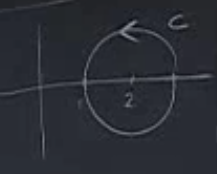
\includegraphics[height=2cm]{22_1.png}

\[ \oint_C ye^{-x} dx + (\frac{1}{2}x^2 - e^{-x})dy \]

Direk olarak

\[ x = 2 + \cos\theta, dx = -\sin\theta \ d\theta \]

\[ y = \sin\theta, dy = \cos\theta \ d\theta \]

Sonra ustteki iki satirdaki formulleri alip entegrale koyardim, ve 0 ile
$\pi$ sinirlari arasinda entegrali hesaplardim. 

Tum bu islemler yerine Green'in Teorisini kullanalim. Yani cift entegral
hesabini yapalim. $M,N$ nedir? 

\[ \oint_C 
\underbrace{ye^{-x}}_{M} dx + 
\underbrace{(\frac{1}{2}x^2 - e^{-x})}_{N}dy \]

Cift entegral o zaman soyle

\[ \int \int_R (N_x - N_y) \ dA =
\]

$R$ nedir? Cemberin icindeki her seydir (cizgili alan). 

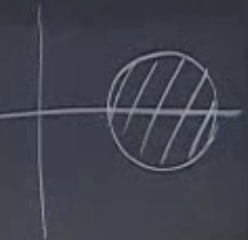
\includegraphics[height=2cm]{22_2.png}

\[=  \int \int_R  \bigg( x+ e^{-x} \bigg) - e^{-x} dA \]

\[=  \int \int_R  x dA \]

Peki bu cift entegrali nasil hesaplayacagiz? Tum cebirsel islemi
yapabiliriz, ya da, bir kisayol dusunelim. 

\[ = Alan(R) \ \bar{x} \]

Cunku cift entegral bir alan hesabi yapiyor. $\bar{x}$ ise $R$ alaninin
yatay eksendeki kutle merkezi, ki ornegimiz icin bu merkez 2
noktasinda. Alan zaten $\pi$, sonuc

\[ = 2\pi \]

Bu arada $\bar{x}$'in tanimi

\[ \bar{x} = \frac{1}{Alan} \int \int x \ dA \]


Simdi Green Teorisinin niye isledigini, yani ispatini gorelim. 

Ozel Durum 

$curl \ \vec{F} = 0$

Bu durumda $\vec{F}$ muhafazakar. 

\[ \oint_C \vec{F} \cdot d\vec{r} = \int \int_R curl \ \vec{F} \ dA \]

Ama curl sifir ise, o zaman sifirin entegrali alinir, bu da sifirdir. 

\[ = 0 \]

Bu ayni zamanda eger kapali egri icindeki her noktada $curl \ \vec{F} = 0$ ise, o
zaman $\oint_C \vec{F} \cdot d\vec{r} = 0$ oldugunun ispatidir, bu da $\vec{F}$'in muhafazakar oldugunun
ispatidir. 

Problem Set 8 Problem 2 icin Green Teorisi uygulanamiyor, cunku $C$
icinde orijin var. 

Ispat

Sunu ispatlamaya ugrasiyoruz

\[ \oint_C M dx + N dy = \int \int_R (N_x - M_y) \ dA \]

Isimizi kolaylastirmak icin daha basit bir ifadeyi ispat edelim. Ustteki
formulun ozel bir hali

\[ \oint_C M dx  = \int \int_R -M_y \ dA \]

bu durumda $N=0$, ve vektor alaninda sadece $x$ bileseni var. 

Peki bu ozel sart niye yeterli? Iddia o ki eger bu daha basit ifadeyi ispat
edebilirsem, sadece $y$ bilesenin oldugu diger sarti da ispat edebilirim,
sonra bu iki ozel sarti toplarsam genel sarti elde ederim. 

Diger ozel sart

\[ \oint_C N dy  = \int \int_R N_x \ dA \]

Bir problem daha var, eger egri cetrefil ise cift entegrali olusturmak zor
olabilir. 

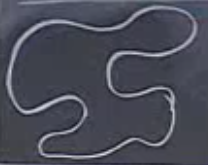
\includegraphics[height=2cm]{22_3.png}

O zaman daha basit egrilerle ise baslamak daha iyi. 

Bir diger gozlem daha, $R$'i daha basit bolgelere ayirabiliriz. 

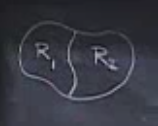
\includegraphics[height=3cm]{22_4.png}

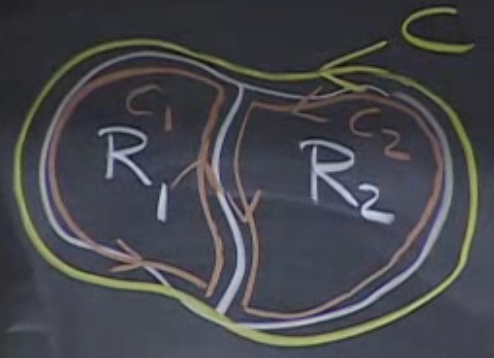
\includegraphics[height=3cm]{22_5.png}

Eger 

\[ \oint_{c_1} M dx  = \int \int_{R_1} -M_y \ dA \]

\[ \oint_{c_2} M dx  = \int \int_{R_2} -M_y \ dA \]

ifadelerinin dogru oldugunu ispatlarsam, o zaman $C$ icin olan ifadenin
dogrulugunu ispatlayabilirim, cunku ustteki iki formulu toplayabilirim. 

Peki ustteki iki formulde sol taraf toplandiginda $R$ bolgesini kabaca
ortadan bolen egriyi iki kere toplamis olmaz miyim? Aslinda evet, ama o
egri uzerindeki gidisata dikkat, biri yukari, digeri asagi yonde. O zaman o
parca iki kere toplaninca birbirlerini iptal edecekler ve sonuc sifir olacak.

O zaman 

\[ \oint_C M dx = \oint_{C_1} + \oint_{C_2} =
\int \int_{R_1} + \int \int_{R_2} = 
\int \int_R -M_ydA
\]

Ornek olarak soyle bir sekli alalim. Bu sekli dikey ve ``basit'' olarak ve
5 parcaya boluyoruz.

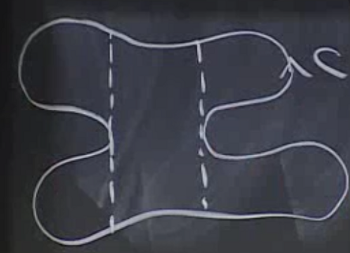
\includegraphics[height=2cm]{22_6.png}

Bu demek? 

\[ a < x < b, \ f_1(x) < y < f_2(x) \]

Kesik cizgilerin x bilesenini $a,b$ olarak alirsak, bu noktalarin $y$
degerleri de dikey (kesik) cizgiler arasinda kaliyor. 

Ana Islem

Eger $R$ dikey ve basit ise, ve $C$, saat yonu tersi olmak uzere $R$'nin
sinirini olusturuyorsa, 

\[ \oint_C M dx  = \int \int_R -M_y \ dA \]

ifadesini ispatla. 

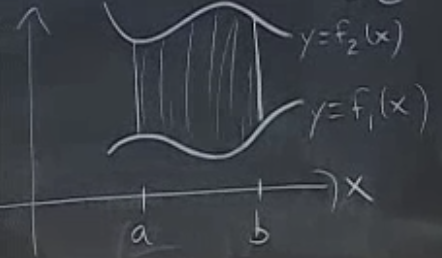
\includegraphics[height=3cm]{22_7.png}

Ustteki de basit olarak bolunmus bir bolgeyi gosteriyor. Cizgili bolumu
nasil hesaplariz?

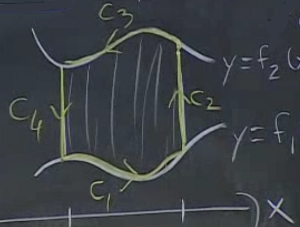
\includegraphics[height=3cm]{22_8.png}

Egriyi 4 parcaya ayiririz. 

$C_1$

\[ y = f_1(x) \]

$x$ degeri $a$'dan $b$'ye gidiyor. 

\[ \int_{c_1}M(x,y) dx = \int_a^b M(x,f_1(x))  dx\]

Burada tek degisken uzerinden entegral alabilirim. Tabii bu ispatta $M$
ifadesini bilmedigim icin bunu yapamam, tanimi burada birakirim. 

$C_2$

$x$ degeri $b$, $dx = 0$

\[ \int_{c_2}M(x,y) dx = 0\]

Ayni sekilde $C_4$ sifir olur. 

$C_3$

\[ y = f_2(x) \]

$x$ degeri $b$'dan $a$'ya gidiyor. 

\[ \int_{c_2}M(x,y) dx = \int_b^a M(x,f_2(x)) dx = 
-  \int_a^b M(x,f_2(x)) dx 
\]

Hepsini toplarsak

\[ \oint_C M dx  =
\int_a^b M(x,f_1(x))  dx -
\int_a^b M(x,f_2(x)) dx 
\mlabel{1}
 \]

Simdi cift entegrale bakiyorum, ve bakalim bu cift entegrali ustteki
ifadeye esitleyebilecek miyim. 

\[ \int \int_R -M_y dA = 
- \int_a^b \int_{f_1(x)}^{f_2(x)} \frac{\partial M}{\partial y} dy dx \]

Daha once soylemistik, bolgeyi belli basit, belli bir sekilde secmemizin
sebebi $dy,dx$'i ayarlamamizin kolay olmasi icindi. Yani cift entegral icin
kesitler hazirlarken bu kesitlerin kolay olmasi icin bolgeyi boyle
sectik. 

Icteki entegral

\[ \int_{f_1(x)}^{f_2(x)} \frac{\partial M}{\partial y} dy =
M(x,f_2(x)) - M(x,f_1(x))
 \]

Geri koyarsak

\[ \int \int_R -M_y dA = 
- \int_a^b M(x,f_2(x)) - M(x,f_1(x)) dx \]

Bu ifade (1) ifadesi ile ayni. Ispat tamamlandi. Cunku ozel sart dikeysel
basit bolgelerde ispat gecerli, bu faraziyeyi ortadan kaldirirsak, tum
bolgeler icin ispat gecerli. $y$ bileseni icin de ayni sey gecerli, o zaman
genel teori ispatlanmis oldu.

Guzel Bir Ornek 

Green'in Teorisi icin bir ornek sudur. Bilgisayarlar bu kadar yaygin olmadan
once deneysel fizikciler deneylerden sonra bir kagit, duzey uzerinde
deneylerinin sonuclarini baski halinde alirlardi. Bu noktalar belli
bolgede, bir egri icinde olurdu. Fakat bu bolgenin alani lazimdi, bu hesap
nasil yapilacakti?

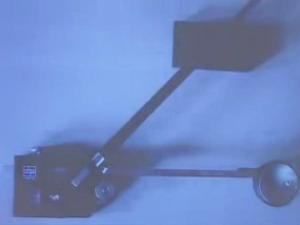
\includegraphics[height=4cm]{22_9.png}

Ustteki planimeter denen alet buna yariyordu. Kollardan birini alttaki gibi
bir cikti uzerinde, onun egrileri uzerinde gezdirip, basladiginiz noktaya
donunce, alet pat diye size hemen sonucu soyluyordu. Nasil ?

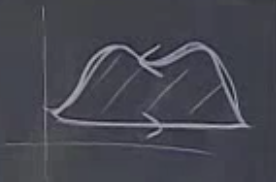
\includegraphics[height=2cm]{22_10.png}

Bunu cizgisel entegrali hesaplayarak yapiyordu. Green'in Teorisine gore
cizgisel entegral, alani iceren entegrale esit oldugu icin dogru sonucu
veriyordu.

\[ \oint_C x \ dy  = \int \int_R 1 \ dA = Alan(R) \]

Alet esitligin solundaki hesabi yapiyor, bize aradigimiz sagdaki sonucu
veriyordu yani. 

Eger aletin nasil isledigi hakkinda bir spekulasyon yapmak gerekirse,
vektor alani $x$'i ele alalim (cizmek icin gerekli kod ile)

\begin{minted}{python}
x = linspace(0,10.,10)
y = linspace(0,10.,10)
x,y = meshgrid(x,y)
u = x*10
v = np.zeros(y.shape)
q = plt.quiver(x,y,u,v,angles='xy',scale=1000,color='r')
p = plt.quiverkey(q,1,16.5,50,"50 m/s",coordinates='data',color='r')
plt.savefig('field_x.png')
\end{minted}

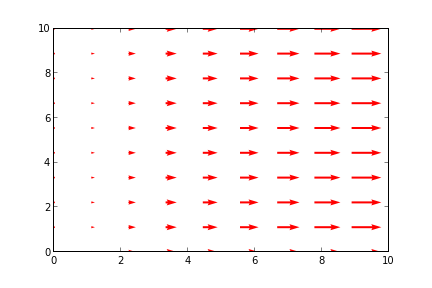
\includegraphics[height=4cm]{field_x.png}

Bu vektorler mekanik alet icinde belki teller, ya da demir cubuklar olarak
gosteriliyor olabilir. Hareket ettirilen kol, kadran gezdirilirken ``dikey
hareket farki'' yani $dy$ bir sekilde aliniyor (belki de isi basitlestirmek
icin onceden tanimli bir sabit olarak kabul edildi), sonra gezdirilme
sirasinda hangi tele (vektore) ``carpildiysa'' dikey fark bu vektorun
degeri ile bir sekilde carpilip, baska bir mekanik bilesende
toplaniyor. Basa donulunce eldeki toplam aranan alan degeri olacaktir.

Not: Enb asit ok cizimi icin alttaki kod kullanilabilir

\begin{minted}{python}
u = 200
v = 200
q = plt.quiver(10,10,u,v,angles='xy',scale=1000,color='r')
p = plt.quiverkey(q,1,16.5,50,"50 m/s",coordinates='data',color='r')
xl = plt.xlabel("x (km)")
yl = plt.ylabel("y (km)")
\end{minted}



\end{document}
